\documentclass{article}
\usepackage[final,main]{neurips_2025}  % "main" track option required by the .sty in camera-ready mode  % NEURIPS style

\usepackage[utf8]{inputenc}
\usepackage[T1]{fontenc}
\usepackage[hidelinks]{hyperref}  % clickable links
\usepackage{booktabs}
\usepackage{graphicx}
\usepackage{amsmath,amssymb}
\usepackage{subcaption}
\usepackage{multirow}
\usepackage{enumitem}
\usepackage{xspace}
\usepackage{natbib}
\usepackage{algorithm}
\usepackage[noend]{algpseudocode}

% Import command files
\input{commands/math}
\input{commands/general}
%%%%% PROJECT-SPECIFIC MACROS %%%%%
% Terms used throughout this paper. Import with: %%%%% PROJECT-SPECIFIC MACROS %%%%%
% Terms used throughout this paper. Import with: %%%%% PROJECT-SPECIFIC MACROS %%%%%
% Terms used throughout this paper. Import with: \input{commands/macros}

\usepackage{xspace}

%%%%%%%%%%%%%%%%%%%%%%%%%%%%%%%%%%%%%%%%%%%%%%%%%%%%%%%%%%%%%%%%%
% SIGNALS UNDER STUDY
%%%%%%%%%%%%%%%%%%%%%%%%%%%%%%%%%%%%%%%%%%%%%%%%%%%%%%%%%%%%%%%%%

\newcommand{\plddt}{\textsc{pLDDT}\xspace}
\newcommand{\afplddt}{\textsc{AlphaFold-pLDDT}\xspace}
\newcommand{\afrsa}{\textsc{AlphaFold-rsa}\xspace}
\newcommand{\afthreeplddt}{\textsc{AlphaFold3-pLDDT}\xspace}
\newcommand{\afthreersa}{\textsc{AlphaFold3-rsa}\xspace}
\newcommand{\rsa}{\textsc{RSA}\xspace}
\newcommand{\plddtrule}{\textsc{pLDDT}$<$50\xspace}

%%%%%%%%%%%%%%%%%%%%%%%%%%%%%%%%%%%%%%%%%%%%%%%%%%%%%%%%%%%%%%%%%
% DATASET NAMES
%%%%%%%%%%%%%%%%%%%%%%%%%%%%%%%%%%%%%%%%%%%%%%%%%%%%%%%%%%%%%%%%%

\newcommand{\caidtwo}{\textsc{CAID2}\xspace}
\newcommand{\caidthree}{\textsc{CAID3}\xspace}
\newcommand{\dpdb}{\textsc{Disorder-PDB}\xspace}
\newcommand{\dnox}{\textsc{Disorder-NOX}\xspace}
\newcommand{\disprot}{\textsc{DisProt}\xspace}
\newcommand{\afdb}{\textsc{AlphaFold DB}\xspace}

%%%%%%%%%%%%%%%%%%%%%%%%%%%%%%%%%%%%%%%%%%%%%%%%%%%%%%%%%%%%%%%%%
% CLAUSE LABELS
%%%%%%%%%%%%%%%%%%%%%%%%%%%%%%%%%%%%%%%%%%%%%%%%%%%%%%%%%%%%%%%%%

\newcommand{\cone}{\textbf{C1}\xspace}
\newcommand{\ctwo}{\textbf{C2}\xspace}
\newcommand{\cthree}{\textbf{C3}\xspace}
\newcommand{\cfour}{\textbf{C4}\xspace}

%%%%%%%%%%%%%%%%%%%%%%%%%%%%%%%%%%%%%%%%%%%%%%%%%%%%%%%%%%%%%%%%%
% ABBREVIATIONS
%%%%%%%%%%%%%%%%%%%%%%%%%%%%%%%%%%%%%%%%%%%%%%%%%%%%%%%%%%%%%%%%%

\newcommand{\idr}{IDR\xspace}
\newcommand{\idrs}{IDRs\xspace}
\newcommand{\bacc}{BACC\xspace}
\newcommand{\pp}{\,pp\xspace}
\newcommand{\ie}{i.e.,\xspace}
\newcommand{\eg}{e.g.,\xspace}


\usepackage{xspace}

%%%%%%%%%%%%%%%%%%%%%%%%%%%%%%%%%%%%%%%%%%%%%%%%%%%%%%%%%%%%%%%%%
% SIGNALS UNDER STUDY
%%%%%%%%%%%%%%%%%%%%%%%%%%%%%%%%%%%%%%%%%%%%%%%%%%%%%%%%%%%%%%%%%

\newcommand{\plddt}{\textsc{pLDDT}\xspace}
\newcommand{\afplddt}{\textsc{AlphaFold-pLDDT}\xspace}
\newcommand{\afrsa}{\textsc{AlphaFold-rsa}\xspace}
\newcommand{\afthreeplddt}{\textsc{AlphaFold3-pLDDT}\xspace}
\newcommand{\afthreersa}{\textsc{AlphaFold3-rsa}\xspace}
\newcommand{\rsa}{\textsc{RSA}\xspace}
\newcommand{\plddtrule}{\textsc{pLDDT}$<$50\xspace}

%%%%%%%%%%%%%%%%%%%%%%%%%%%%%%%%%%%%%%%%%%%%%%%%%%%%%%%%%%%%%%%%%
% DATASET NAMES
%%%%%%%%%%%%%%%%%%%%%%%%%%%%%%%%%%%%%%%%%%%%%%%%%%%%%%%%%%%%%%%%%

\newcommand{\caidtwo}{\textsc{CAID2}\xspace}
\newcommand{\caidthree}{\textsc{CAID3}\xspace}
\newcommand{\dpdb}{\textsc{Disorder-PDB}\xspace}
\newcommand{\dnox}{\textsc{Disorder-NOX}\xspace}
\newcommand{\disprot}{\textsc{DisProt}\xspace}
\newcommand{\afdb}{\textsc{AlphaFold DB}\xspace}

%%%%%%%%%%%%%%%%%%%%%%%%%%%%%%%%%%%%%%%%%%%%%%%%%%%%%%%%%%%%%%%%%
% CLAUSE LABELS
%%%%%%%%%%%%%%%%%%%%%%%%%%%%%%%%%%%%%%%%%%%%%%%%%%%%%%%%%%%%%%%%%

\newcommand{\cone}{\textbf{C1}\xspace}
\newcommand{\ctwo}{\textbf{C2}\xspace}
\newcommand{\cthree}{\textbf{C3}\xspace}
\newcommand{\cfour}{\textbf{C4}\xspace}

%%%%%%%%%%%%%%%%%%%%%%%%%%%%%%%%%%%%%%%%%%%%%%%%%%%%%%%%%%%%%%%%%
% ABBREVIATIONS
%%%%%%%%%%%%%%%%%%%%%%%%%%%%%%%%%%%%%%%%%%%%%%%%%%%%%%%%%%%%%%%%%

\newcommand{\idr}{IDR\xspace}
\newcommand{\idrs}{IDRs\xspace}
\newcommand{\bacc}{BACC\xspace}
\newcommand{\pp}{\,pp\xspace}
\newcommand{\ie}{i.e.,\xspace}
\newcommand{\eg}{e.g.,\xspace}


\usepackage{xspace}

%%%%%%%%%%%%%%%%%%%%%%%%%%%%%%%%%%%%%%%%%%%%%%%%%%%%%%%%%%%%%%%%%
% SIGNALS UNDER STUDY
%%%%%%%%%%%%%%%%%%%%%%%%%%%%%%%%%%%%%%%%%%%%%%%%%%%%%%%%%%%%%%%%%

\newcommand{\plddt}{\textsc{pLDDT}\xspace}
\newcommand{\afplddt}{\textsc{AlphaFold-pLDDT}\xspace}
\newcommand{\afrsa}{\textsc{AlphaFold-rsa}\xspace}
\newcommand{\afthreeplddt}{\textsc{AlphaFold3-pLDDT}\xspace}
\newcommand{\afthreersa}{\textsc{AlphaFold3-rsa}\xspace}
\newcommand{\rsa}{\textsc{RSA}\xspace}
\newcommand{\plddtrule}{\textsc{pLDDT}$<$50\xspace}

%%%%%%%%%%%%%%%%%%%%%%%%%%%%%%%%%%%%%%%%%%%%%%%%%%%%%%%%%%%%%%%%%
% DATASET NAMES
%%%%%%%%%%%%%%%%%%%%%%%%%%%%%%%%%%%%%%%%%%%%%%%%%%%%%%%%%%%%%%%%%

\newcommand{\caidtwo}{\textsc{CAID2}\xspace}
\newcommand{\caidthree}{\textsc{CAID3}\xspace}
\newcommand{\dpdb}{\textsc{Disorder-PDB}\xspace}
\newcommand{\dnox}{\textsc{Disorder-NOX}\xspace}
\newcommand{\disprot}{\textsc{DisProt}\xspace}
\newcommand{\afdb}{\textsc{AlphaFold DB}\xspace}

%%%%%%%%%%%%%%%%%%%%%%%%%%%%%%%%%%%%%%%%%%%%%%%%%%%%%%%%%%%%%%%%%
% CLAUSE LABELS
%%%%%%%%%%%%%%%%%%%%%%%%%%%%%%%%%%%%%%%%%%%%%%%%%%%%%%%%%%%%%%%%%

\newcommand{\cone}{\textbf{C1}\xspace}
\newcommand{\ctwo}{\textbf{C2}\xspace}
\newcommand{\cthree}{\textbf{C3}\xspace}
\newcommand{\cfour}{\textbf{C4}\xspace}

%%%%%%%%%%%%%%%%%%%%%%%%%%%%%%%%%%%%%%%%%%%%%%%%%%%%%%%%%%%%%%%%%
% ABBREVIATIONS
%%%%%%%%%%%%%%%%%%%%%%%%%%%%%%%%%%%%%%%%%%%%%%%%%%%%%%%%%%%%%%%%%

\newcommand{\idr}{IDR\xspace}
\newcommand{\idrs}{IDRs\xspace}
\newcommand{\bacc}{BACC\xspace}
\newcommand{\pp}{\,pp\xspace}
\newcommand{\ie}{i.e.,\xspace}
\newcommand{\eg}{e.g.,\xspace}


\captionsetup[table]{aboveskip=4pt,belowskip=4pt}
\captionsetup[figure]{aboveskip=4pt,belowskip=4pt}
\captionsetup[subfigure]{aboveskip=2pt,belowskip=2pt}

\bibliographystyle{plainnat}

\title{Is \texorpdfstring{pLDDT $<$ 50}{pLDDT < 50} a Disorder Detector?\\
An Operating-Point Audit of AlphaFold2 Confidence Against Experimental Disorder Annotations}

\author{NeuriCo}

\begin{document}

\maketitle

\begin{abstract}
AlphaFold DB covers more than 200 million proteins, and the rule ``\plddt $<$ 50 means
intrinsically disordered'' has become an everyday working heuristic for trimming models and
annotating the dark proteome. The rule has never been validated at the operating point at
which it is used: the literature reports ROC-AUC, a threshold-free summary that cannot
adjudicate a claim about a specific cutoff. We audit the rule directly on the CAID round-2 and
round-3 blind assessments, across both official reference conventions (\dpdb and \dnox), with
bootstrap confidence intervals over targets and coverage-matched target sets, against a panel
of 37--56 dedicated disorder predictors. We find that \plddtrule has sensitivity 0.60--0.63
(0.63--0.65 restricted to regions longer than 30 residues), not above 0.8: not one of 1000
bootstrap resamples reaches 0.80 in any of four settings. Its specificity is 0.98 under \dpdb
and 0.67--0.76 under \dnox --- a 30-point swing produced entirely by how the benchmark defines
a negative, not by AlphaFold. Once every method is threshold-calibrated, none of 174
method\,$\times$\,dataset comparisons beats \plddt on short ($<$20 aa) segments, and the median
dedicated predictor is 1.5--8.7 points \emph{worse}; the widely assumed 10--15\% advantage is
exactly reproducible at a shared naive 0.5 cut and vanishes after calibration. What survives is
the mechanism: reading solvent accessibility out of the \emph{same} AlphaFold2 coordinates is
significantly better on every reference set ($\Delta$AUC $+0.015$ to $+0.056$, all $p \le 0.02$),
and the disorder \plddt misses is confidently modelled and solvent-exposed.
\plddtrule is a high-precision, low-recall detector; users who need recall should raise the
cutoff to $\approx$70 and prefer the geometric readout of the same model.

\end{abstract}

\section{Introduction}
\label{sec:intro}

AlphaFold2 attaches a per-residue confidence score, \plddt, to every model it
builds~\citep{jumper2021}. Almost immediately after the human proteome was released, it was
noticed that regions with low \plddt line up strikingly well with known intrinsically
disordered regions (\idrs)~\citep{tunyasuvunakool2021}. That observation hardened into a rule
of thumb: \emph{pLDDT $<$ 50 means disordered}. The rule is now used every day to trim models,
to annotate the dark proteome, and to nominate \idr candidates for experiment, across a database
of more than 200 million structures~\citep{varadi2022}. If it is miscalibrated, the error
propagates silently into every study that adopts it.

\para{The rule has never been checked where it is used.} Prior evaluations of \plddt as a
disorder signal report ROC-AUC~\citep{piovesan2022,kurgan2023}. AUC is threshold-free, and a
threshold-free summary is structurally incapable of adjudicating a claim about a specific
cutoff. Nobody has reported the sensitivity and specificity of the literal \plddtrule cut,
stratified by region length, on both of the reference conventions that the community's own
blind assessment publishes. That is the gap we fill.

\para{What exactly is being claimed?} The folk rule comes bundled with a set of quantitative
expectations that are worth writing down and testing separately. We decompose the standard
framing into four claims: \cone the rule finds long ($>$30 aa) \idrs with sensitivity above
0.8; \ctwo its specificity is below 0.7; \cthree it works this way because \plddt conflates
conformational flexibility with prediction uncertainty; and \cfour dedicated disorder
predictors achieve 10--15\% better balanced accuracy on short ($<$20 aa) disordered segments.
Each clause implies a different remedy, so each deserves its own measurement.

\para{Our approach.} We do not train or run a new predictor. The CAID blind
assessments~\citep{delconte2023,mehdiabadi2026} already contain the experimental ground truth
(derived from \disprot~\citep{quaglia2022}) and the per-residue outputs of every participating
method, \emph{including the official AlphaFold-pLDDT baseline that the rule refers to}. We evaluate
that baseline at the exact operating point in question, on all four combinations of CAID round
(2, 3) and reference convention (\dpdb, \dnox), with bootstrap confidence intervals resampled
over targets, coverage-matched target sets, and three distinct threshold conventions for every
comparator (\figref{fig:clause}). We additionally re-parse 588 \afdb models to characterise,
structurally, the residues the rule gets wrong.

\para{What we find.} Three of the four clauses are false and one is right.
Sensitivity is $0.60$--$0.63$, and $0.63$--$0.65$ on long regions --- $P(\text{sens} \ge 0.80) =
0.000$ in every setting (\cone falsified). Specificity is $0.98$ under \dpdb and $0.67$--$0.76$
under \dnox, so \ctwo describes an annotation convention rather than a predictor. After fair
threshold calibration, \emph{zero} of 174 method\,$\times$\,dataset comparisons beat \plddt on
short segments and the median comparator is $1.5$--$8.7$ percentage points worse, yet the very
same claim is exactly reproducible at a shared naive 0.5 cut, where 9 of 52 predictors land
inside the hypothesised $+10$ to $+15$\pp band (\cfour falsified, and diagnosed as a
calibration artefact). The mechanism clause survives four independent tests: solvent
accessibility read from the same coordinates beats \plddt by $+0.015$ to $+0.056$ AUC
($p \le 0.02$ everywhere), a stronger folding model does not improve \plddt, \plddt is near
chance \emph{within} its own low band (AUC $0.44$--$0.63$) where geometry still separates
disorder at $0.56$--$0.83$, and the disorder the rule misses is confidently modelled
(mean \plddt 70--74) and solvent-exposed (mean RSA $0.46$--$0.51$).

\para{Contributions.}
\begin{itemize}[leftmargin=*,itemsep=0pt,topsep=2pt]
    \item We report the first operating-point-resolved evaluation of the literal \plddtrule
    rule --- sensitivity, specificity, balanced accuracy and MCC with bootstrap CIs --- on all
    four CAID round $\times$ reference-convention combinations, and show the rule is
    high-precision and low-recall, missing $\approx$40\% of annotated disorder.
    \item We stratify \emph{regions} (not proteins) into $<$20 / 20--30 / $>$30 aa bins under
    two explicitly stated definitions of ``balanced accuracy on short segments'', and show that
    no dedicated predictor significantly beats \plddt there once thresholds are calibrated.
    \item We diagnose the widely believed short-segment advantage as a threshold-calibration
    artefact, reproducing it exactly at a shared 0.5 cut and dissolving it under calibration ---
    a methodological warning that generalises beyond disorder prediction.
    \item We test the conflation mechanism with the structure model held fixed, comparing
    \plddt against solvent accessibility of the same AlphaFold2 coordinates, and characterise
    the missed disorder as exposed pseudostructure rather than conditional folding.
\end{itemize}

\secref{sec:related} places the work against prior evaluations, \secref{sec:method} describes
the data, panel, operating points and statistics, \secref{sec:results} reports the four clause
tests, and \secref{sec:discussion} discusses limitations and practical consequences.

\section{Related Work}
\label{sec:related}

\para{AlphaFold confidence as a disorder signal.} \citet{jumper2021} introduced \plddt as a
predicted lDDT-C$\alpha$ against the unknown true structure, and \citet{tunyasuvunakool2021}
reported the correlation between low-confidence regions and known \idrs at proteome scale.
\citet{piovesan2022} turned that correlation into concrete, evaluable baselines:
\afplddt with score $=1-\plddt/100$, and \afrsa, the DSSP relative solvent accessibility of the
same model smoothed over a 25-residue window. These are the definitions CAID has used ever
since, and the first of them is exactly the object of the folk rule --- score $>0.50$ is
identically \plddtrule. \citet{wilson2022} asked early whether \plddt should be used as a
disorder predictor at all and cautioned that a real correlation does not make the semantics the
same. All of this work reports AUC. Unlike these studies, we evaluate the baseline at the
specific cutoff practitioners actually apply.

\para{Blind assessment of disorder predictors.} CAID~\citep{necci2021} established the
evaluation protocol we inherit: \disprot-derived references~\citep{quaglia2022}, per-residue
scores, blind submission, bootstrap over targets. Round 2~\citep{delconte2023} was the first to
include the AlphaFold baselines as official entries; round 3~\citep{mehdiabadi2026} added 24
methods, reported that protein language models now lead, and noted that \afplddt ranks 11th
while \afthreeplddt ranks 13th on \dpdb. CAID publishes two disorder references that differ
\emph{only} in how a negative is defined: \dpdb counts as negative only residues observed in an
experimental PDB structure, whereas \dnox counts every non-annotated residue as negative. CAID3
quantifies the divergence (57.3\% vs 23.9\% positive content on shared proteins) but treats it
as a caveat. We treat it as the dominant term in specificity and report every result under both
conventions.

\para{The closest prior comparison.} \citet{kurgan2023} is the nearest work to ours: 20
comparators on CAID1, AF2-\plddt at AUC 0.722 against flDPnn~\citep{hu2021} at 0.814 and
AF2-RSA at 0.768, with a long ($>$30) versus short ($\le$30) \idr split. Two features of that
design leave our questions open. Their split is at the \emph{protein} level --- proteins whose
\idrs are all short --- rather than at the region level, so the $<$20 aa region bin named in the
folk rule is unexamined; and their metric is AUC, so no operating point is adjudicated. They
also state the conflation mechanism informally, observing that low \plddt could mean the
structure space is poorly covered \emph{or} that the segment is disordered, while unusually high
solvent accessibility ``seems to be a better proxy'' for disorder. Building on that observation,
we turn it into a controlled test: same coordinates, two readouts, paired bootstrap. We also
adopt their content-matched calibration as one of our three operating points.

\para{What low confidence actually means.} \citet{richardson2025} partition low-\plddt residues
into barbed wire, pseudostructure, near-predictive and unphysical modes, and find that the
barbed-wire and near-predictive curves cross near \plddt 50 --- so a cut at 50 cleanly removes
non-predictive residues but cannot separate pseudostructure. Symmetrically,
\citet{alderson2023} show that \idrs which conditionally fold are modelled with \emph{high}
\plddt. Both halves of the conflation are therefore documented in the literature; what is
missing is a measurement of how much of the rule's error each half accounts for. We supply that
decomposition. Supporting mechanistic work reports that \plddt tracks dynamics rather than model
error alone~\citep{guo2022}, and that AlphaFold2 collapses conformational heterogeneity to a
single state~\citep{chakravarty2022,bhattacharya2022}.

\para{Threshold calibration in method comparison.} \citet{kurgan2023} explicitly calibrate
binary predictions to reproduce the correct number of disordered residues, and CAID reports
threshold-free metrics precisely because submitted scores are not mutually calibrated. Our
\cfour analysis shows what happens when this discipline is dropped: the comparison at a shared
0.5 cut is not a comparison of methods but of operating points, and it produces a specific,
reproducible, and wrong quantitative conclusion.

\section{Methodology}
\label{sec:method}

\subsection{Problem statement and design}
\label{sec:setup}

We test an evaluation claim about a fixed operating point, so the right instrument is an
existing blind benchmark rather than a new prediction run. Let $s_m(r) \in [0,1]$ be method
$m$'s disorder score for residue $r$ and $y(r) \in \{0,1\}$ the experimental label. The rule
under audit is the classifier $\hat{y}(r) = \mathbb{1}[\plddt(r) < 50]$, which under the CAID
encoding $s_{\afplddt} = 1 - \plddt/100$~\citep{piovesan2022} is identically
$\mathbb{1}[s(r) > 0.5]$. Nothing has to be re-predicted: the CAID archives contain both the
ground truth and the official \afplddt submission. We downloaded AlphaFold2 coordinates
separately only to characterise the errors structurally and to verify that the CAID scores
really are $1 - \plddt/100$.

Four design decisions each answer a specific way the result could have been an artefact.
\emph{(i)} Specificity depends entirely on how negatives are defined, so both CAID references
are reported for every result and neither is treated as ``the'' answer. \emph{(ii)} AlphaFold
covers only 82--86\% of CAID2 targets while other methods cover $\approx$100\%, so every
comparison runs on the intersection of targets covered by all panel methods; the \cone/\ctwo
tests are additionally repeated on \plddt's own coverage and on the full reference with missing
targets scored as all-ordered. \emph{(iii)} Comparing all methods at a shared 0.5 cut is
meaningful only for \plddt, so every method is evaluated at three operating points.
\emph{(iv)} Choosing a threshold on the data one then scores is optimistically biased, so the
optimism is measured directly by repeated cross-validation and reported.

\subsection{Data}

We use the four CAID disorder reference sets (\tabref{tab:data}). The two conventions differ
only in the definition of a negative: \dpdb counts as negative only residues observed in an
experimental PDB structure, excluding X-ray-missing residues (hence the large excluded column);
\dnox counts every non-annotated residue as negative. We identified which CAID release each
downloaded reference corresponds to by exact matching on (\#sequences, positives, negatives,
undefined) against the four official reference-set manifests; CAID3 turns out to be the v3
round, so all official comparisons use the v3 files.

\begin{table}[t]
    \centering
    \small
    \begin{tabular}{@{}lrrrrl@{}}
        \toprule
        \textbf{Reference set} & \textbf{Targets} & \textbf{Positives} & \textbf{Negatives} &
        \textbf{Excluded} & \textbf{Release} \\
        \midrule
        \caidtwo \dpdb   & 348 & 37,072 & 93,805 & 156,143 & CAID2 \\
        \caidtwo \dnox   & 210 & 31,315 & 129,487 & 0 & CAID2 \\
        \caidthree \dpdb & 319 & 31,401 & 67,838 & 61,183 & CAID3 v3 \\
        \caidthree \dnox & 204 & 26,367 & 73,610 & 541 & CAID3 v3 \\
        \bottomrule
    \end{tabular}
    \caption{The four evaluation references. Residue counts are as published by CAID. The
    ``Excluded'' column holds residues with no evidence either way; \dpdb discards them, \dnox
    treats almost all of them as ordered. This single convention difference drives the
    specificity result in \secref{sec:c2}.}
    \label{tab:data}
\end{table}

We additionally re-parsed 588 \afdb models (94\% of mappable CAID targets) into per-residue
\plddt and Shrake--Rupley relative solvent accessibility for the structural error analysis.

\subsection{Comparator panel and operating points}

\para{Panel.} We restrict the panel to \emph{general} intrinsic-disorder predictors: 37 methods
on \caidtwo and 56 on \caidthree. It spans classical
predictors (IUPred3~\citep{erdos2021}, ESpritz-D~\citep{walsh2012},
MobiDB-lite~\citep{necci2017,piovesan2025}, VSL2, RONN, DisEMBL), strong sequence-based methods
(flDPnn~\citep{hu2021}, AIUPred, DISOPRED3~\citep{jones2015},
SPOT-Disorder2~\citep{hanson2019}, Metapredict~\citep{emenecker2021}) and protein-language-model
methods (PUNCH2, SETH~\citep{ilzhofer2022}, DisorderUnetLM, ESMDisPred, Dispredict3). Methods that predict a different target --- disordered
\emph{binding} regions (ANCHOR2, MoRFchibi, DisoRDPbind, \dots) or linkers --- are excluded,
because including them would flatter \plddt. Two entries (FoldUnfold, NeProc-disorder) submitted
binary states with an empty score column and cannot be threshold-calibrated; they are excluded
and the exclusion is logged. Excluding them is the conservative choice, since at their implicit
0.5 cut they would have added two artificially weak comparators to the \cfour test. AlphaFold-derived
entries (\afplddt, \afrsa, \afthreeplddt, \afthreersa) are tracked separately as the object of
study and its mechanistic controls, leaving 35 and 52 \emph{dedicated} predictors respectively.

\para{Three operating points.} Every method is scored at (a) the \textbf{literal} threshold
$0.5$, which is the only point at which the folk rule is defined; (b) a \textbf{calibrated}
threshold maximising MCC on the reference, which is our primary setting; and (c) a
\textbf{content-matched} threshold reproducing the true number of disordered residues, following
\citet{kurgan2023}. The literal comparison is reported precisely to show how misleading it is.

\subsection{Metrics and statistics}

We compute residue-level sensitivity, specificity, balanced accuracy (\bacc), MCC, precision,
F1 and ROC-AUC, pooled over residues following CAID's ``dataset'' convention. Uncertainty comes
from bootstrap resampling \emph{over targets} (1000 resamples for binary metrics, 500 for AUC),
which is CAID's own resampling unit and respects the fact that residues within a protein are not
independent. All method-vs-\plddt comparisons use a paired bootstrap with identical target
indices for both methods, so the interval is on the difference, with a two-sided bootstrap
$p$-value. Clause tests \cone and \ctwo are one-sided bootstrap probabilities, \eg
$P(\text{sensitivity} \ge 0.80)$ over resamples.

\para{Two definitions of ``balanced accuracy on short segments''.} The folk claim does not define
this quantity, so we compute two and report both. The \textbf{global-negative} (strict)
definition pairs recall over positive residues in 1--19 aa regions with specificity over
\emph{all} evaluated negatives, so a method cannot buy short-region recall with false positives
elsewhere. The \textbf{locally-flanked} (generous) definition scores each region only against
the ordered residues immediately flanking it (up to $\lceil L/2 \rceil$ evaluated negatives per
side), which removes the influence of a method's global false-positive rate entirely. We also
report region-level detection rates --- a region counts as detected when $\ge 25/50/75\%$ of its
evaluated residues are predicted disordered --- since the claim is phrased about regions.

\subsection{Pipeline validation}
\label{sec:validation}

Before running any experiment we validated the pipeline against the official CAID outputs.
For every full-coverage method our pooled AUC reproduces the published value to three decimals
on all four references (\eg IUPred3 0.8854 vs 0.885, ESpritz-D 0.8989 vs 0.899, MobiDB-lite
0.8680 vs 0.868, SETH-1 0.9115 vs 0.911 on \caidtwo \dpdb; flDPnn 0.8609 vs 0.861 on \caidthree
\dpdb). One trap is worth flagging: the official timing file is keyed by software \emph{group}
and reports the group's best member, so the \textsc{AlphaFold-disorder} group value of
0.947--0.95 is \afrsa (ours 0.9443/0.9498), not \afplddt (ours 0.9287/0.9342). Our threshold
sweep matches the official per-threshold specificity to three decimals at every probed
threshold. Finally, parsing \plddt out of the \afdb coordinates and applying $1-\plddt/100$
reproduces the CAID scores at pooled Pearson $r = 0.9925$ over 323,327 residues in 567 targets
(median per-target $r=0.9955$; median residual 1.14 \plddt units), confirming that the submitted
baseline is the standard \plddt. The residual is \afdb release drift between the CAID submission
and our 2026 snapshot; all benchmark results use the official CAID prediction files, so it does
not propagate.

\subsection{Reproducibility}

Python 3.12.8 with numpy 2.5.3, scipy 1.18.1, pandas 3.0.5, scikit-learn 1.9.0, biopython 1.88.
Seed 42 throughout; all bootstrap index matrices are seeded and shared across methods so that
paired comparisons use identical resamples. No model is trained or run --- all predictions were
downloaded --- so the analysis is CPU-only and completes in under 20 minutes of wall clock.
Re-running the length-stratified and mechanism experiments end to end produced byte-identical
output files.

\section{Results}
\label{sec:results}

\begin{figure}[t]
    \centering
    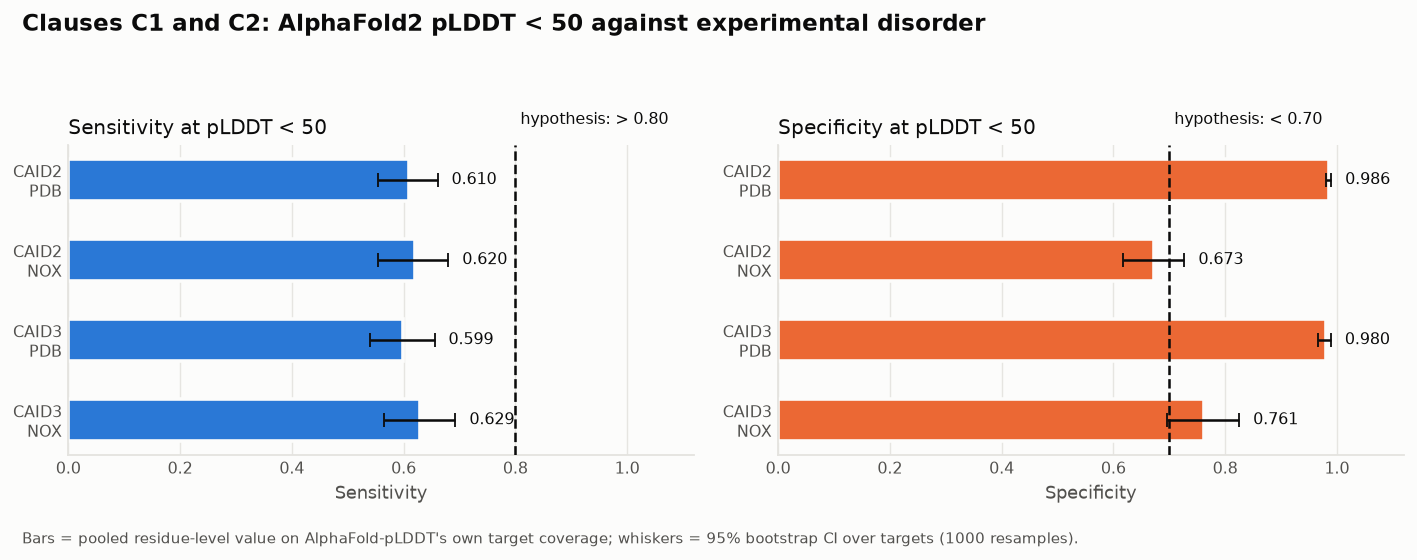
\includegraphics[width=0.95\linewidth]{figures/fig1_clause_verdict.png}
    \caption{Verdicts on the four clauses. Sensitivity of \plddtrule sits at 0.60--0.63 on every
    reference set, far below the claimed 0.8 (dashed line), and restricting to regions longer
    than 30 aa moves it only to 0.63--0.65. Specificity, at the identical operating point,
    is 0.98 under \dpdb and 0.67--0.76 under \dnox: the claim ``specificity $<$ 0.7'' is a
    property of the negative-set convention, not of AlphaFold. Error bars are 95\% bootstrap
    intervals over targets.}
    \label{fig:clause}
\end{figure}

\subsection{C1: sensitivity at \texorpdfstring{\plddtrule}{pLDDT<50} is 0.6, not 0.8}
\label{sec:c1}

\tabref{tab:clause} gives the headline numbers. Sensitivity of the literal rule is
$0.599$--$0.629$ over all disordered residues and $0.630$--$0.648$ restricted to regions longer
than 30 aa. Not one bootstrap resample out of 1000 reached sensitivity 0.80, in any of the four
settings, under either measurement: $P(\text{sens} \ge 0.80) = 0.000$ throughout. The clause
fails by roughly $0.17$ in absolute terms, an order of magnitude larger than the CI half-width.

\begin{table}[t]
    \centering
    \small
    \resizebox{\textwidth}{!}{%
    \begin{tabular}{@{}lrrllrr@{}}
        \toprule
        \textbf{Reference set} & \textbf{$n$} & \textbf{Content} &
        \textbf{Sensitivity (95\% CI)} & \textbf{Sens.\ $>$30 aa} &
        \textbf{Specificity} & \multicolumn{1}{c}{$P(\text{sens}\!\ge\!0.8)$} \\
        \midrule
        \caidtwo \dpdb   & 299 & 0.299 & 0.610 [0.554, 0.661] & 0.634 [0.573, 0.687] & \textbf{0.986} & 0.000 \\
        \caidtwo \dnox   & 173 & 0.235 & 0.620 [0.553, 0.680] & 0.630 [0.562, 0.693] & 0.673 & 0.000 \\
        \caidthree \dpdb & 319 & 0.316 & 0.599 [0.540, 0.655] & 0.630 [0.564, 0.691] & \textbf{0.980} & 0.000 \\
        \caidthree \dnox & 204 & 0.264 & 0.629 [0.565, 0.693] & 0.648 [0.580, 0.711] & 0.761 & 0.000 \\
        \bottomrule
    \end{tabular}}
    \caption{Clause tests for \plddtrule on \plddt's own target coverage. ``Content'' is the
    fraction of evaluated residues that are disordered. Specificity 95\% CIs are
    [0.981, 0.990], [0.618, 0.727], [0.966, 0.989] and [0.696, 0.825] respectively.
    Sensitivity never approaches 0.8; specificity is decided by the reference convention.}
    \label{tab:clause}
\end{table}

\para{The result is not an artefact of the target set.} Sensitivity ranges over $0.51$--$0.63$
across three target-set conventions --- the full-panel intersection, \plddt's own coverage, and
the full reference with AlphaFold's 49 missing \caidtwo targets scored as all-ordered
(\tabref{tab:robustness} in the appendix). The pessimistic convention lowers sensitivity
further; nothing raises it near 0.8.

\para{Where does sensitivity 0.80 live?} \Figref{fig:sweep} answers this directly. Sweeping the
cutoff, sensitivity first reaches 0.80 at \plddt $<$ 75 on both \caidtwo references, \plddt
$<$ 74 on \caidthree \dpdb and \plddt $<$ 68 on \caidthree \dnox. The specificity paid there is
0.94 on \dpdb --- still excellent --- and 0.60--0.76 on \dnox. This is the study's most
actionable single number: \textbf{the rule is set roughly 20 \plddt units too low}. The
MCC-optimal disorder cutoff on this data is \plddt $\approx$ 69--72, and at \plddt $<$ 70
sensitivity is 0.77--0.82 at specificity 0.95 on \dpdb.

\begin{figure}[t]
    \centering
    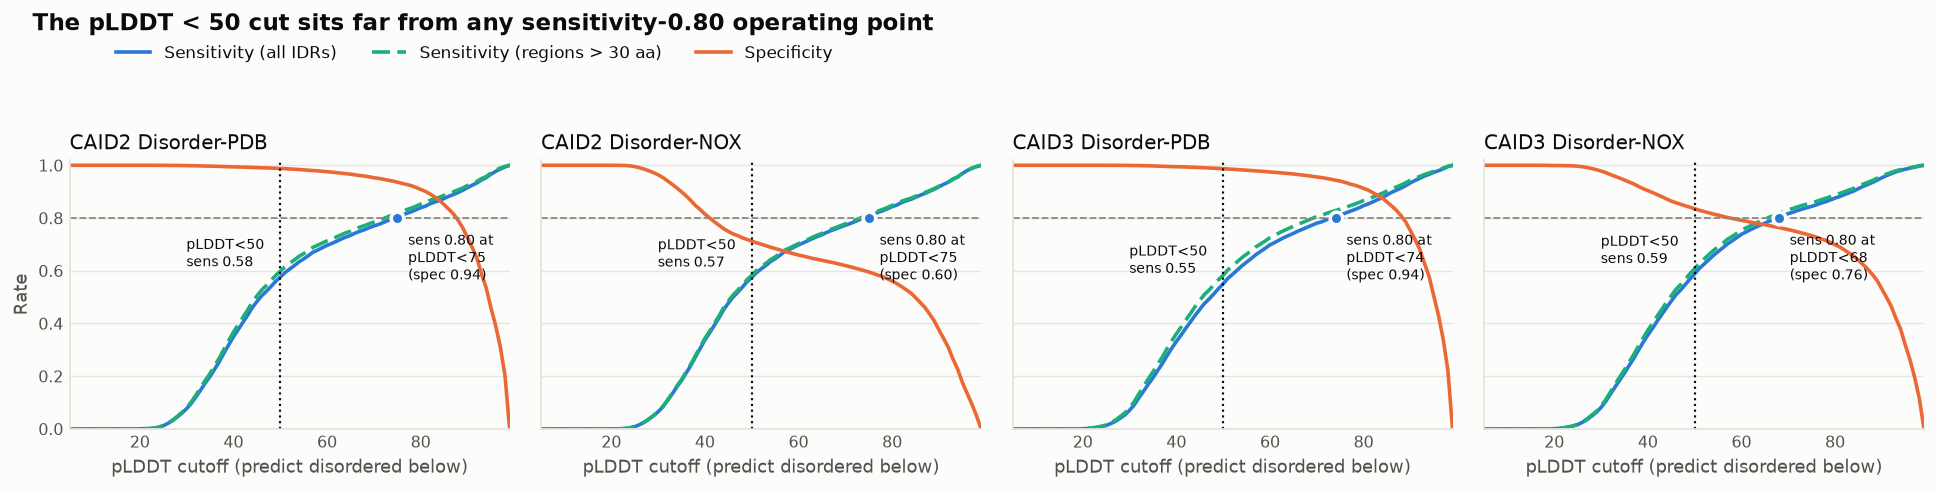
\includegraphics[width=0.95\linewidth]{figures/fig2_cutoff_sweep.png}
    \caption{Sensitivity and specificity of a \plddt cutoff as the cutoff is swept from 5 to 99.
    The vertical line marks the folk rule at 50. The AlphaFold ``very low confidence'' band was
    never calibrated against disorder annotations: on all four references the MCC-optimal
    disorder cutoff falls at \plddt 69--72, and sensitivity 0.80 is not reached until \plddt
    68--75.}
    \label{fig:sweep}
\end{figure}

\subsection{C2: specificity is decided by the negative-set convention}
\label{sec:c2}

At the identical operating point, on the same residues, with the same predictor, specificity is
$0.98$ under \dpdb and $0.67$--$0.76$ under \dnox. The claim ``specificity $<$ 0.7'' is
decisively false on both \dpdb sets ($P(\text{spec} \le 0.70) = 0.000$), consistent with the
data on \caidtwo \dnox ($0.673$, $P = 0.815$), and false on \caidthree \dnox ($0.761$,
$P = 0.032$, \ie significantly \emph{above} 0.7).

The empirical calibration in \tabref{tab:calibration} shows the mechanism. Under \dpdb,
residues in X-ray-missing segments are excluded from the negative set, so almost everything left
below \plddt 50 is a true positive and precision is 0.93--0.95. Under \dnox those same residues
become negatives, and precision collapses to 0.37--0.49 with no change whatsoever in the
predictor. Note the invariant in the last column: \textbf{\plddtrule captures 60--63\% of all
annotated disorder regardless of convention}. That is the stable, method-intrinsic quantity;
what changes is what the complement is called. Recall is the method's property, precision is the
benchmark's.

\begin{table}[t]
    \centering
    \small
    \resizebox{\textwidth}{!}{%
    \begin{tabular}{@{}lrrrrr@{}}
        \toprule
        \textbf{Reference set} & \textbf{Prevalence} & \textbf{\% res.\ \plddt$<$50} &
        $P(\text{dis.}\,|\,\plddt{<}50)$ & $P(\text{dis.}\,|\,\plddt{\ge}50)$ &
        \textbf{Disorder below 50} \\
        \midrule
        \caidtwo \dpdb   & 0.299 & 19.3 & \textbf{0.948} & 0.145 & 0.610 \\
        \caidtwo \dnox   & 0.235 & 39.6 & 0.368 & 0.148 & 0.620 \\
        \caidthree \dpdb & 0.316 & 20.4 & \textbf{0.932} & 0.159 & 0.599 \\
        \caidthree \dnox & 0.264 & 34.1 & 0.486 & 0.149 & 0.629 \\
        \bottomrule
    \end{tabular}}
    \caption{Empirical calibration of the rule. The precision of \plddtrule swings from 0.95 to
    0.37 purely with the negative-set convention, while the share of all annotated disorder that
    falls below \plddt 50 is invariant at 0.60--0.63. Reporting one convention and calling its
    specificity ``the'' specificity is the single most consequential methodological choice in
    this literature.}
    \label{tab:calibration}
\end{table}

\subsection{C4: the short-segment gap is real inside \texorpdfstring{\plddt}{pLDDT}, but dedicated predictors do not close it}
\label{sec:c4}

\para{\plddt does degrade on short regions.} \tabref{tab:strata} shows recall falling from
$0.58$--$0.61$ on regions longer than 30 aa to $0.25$--$0.43$ on regions shorter than 20 aa at
the literal cut. Calibration lifts every stratum but preserves the ordering
($0.59$--$0.65$ short versus $0.78$--$0.85$ long). Region-level detection at 50\% overlap tells
the same story: 59--81\% of short regions detected versus 80--89\% of long ones
(\tabref{tab:regiondetect}, appendix). So the premise behind \cfour --- short disorder is harder
for \plddt --- is correct.

\begin{table}[t]
    \centering
    \small
    \resizebox{\textwidth}{!}{%
    \begin{tabular}{@{}llrrlll@{}}
        \toprule
        \textbf{Reference set} & \textbf{Operating point} & \textbf{Thr.} & \textbf{Spec.} &
        \textbf{Recall $<$20 aa} & \textbf{Recall 20--30 aa} & \textbf{Recall $>$30 aa} \\
        \midrule
        \multirow{2}{*}{\caidtwo \dpdb}   & literal & 0.500 & 0.988 & 0.393 [0.324, 0.457] & 0.485 [0.379, 0.574] & 0.598 [0.537, 0.654] \\
                                          & calibrated & 0.308 & 0.956 & \textbf{0.653} [0.579, 0.721] & 0.691 [0.600, 0.777] & \textbf{0.779} [0.727, 0.827] \\
        \midrule
        \multirow{2}{*}{\caidtwo \dnox}   & literal & 0.500 & 0.712 & 0.433 [0.284, 0.570] & 0.445 [0.307, 0.567] & 0.583 [0.521, 0.651] \\
                                          & calibrated & 0.206 & 0.566 & \textbf{0.806} [0.694, 0.912] & 0.726 [0.571, 0.861] & \textbf{0.844} [0.793, 0.891] \\
        \midrule
        \multirow{2}{*}{\caidthree \dpdb} & literal & 0.500 & 0.987 & 0.331 [0.265, 0.397] & 0.407 [0.316, 0.492] & 0.583 [0.525, 0.637] \\
                                          & calibrated & 0.282 & 0.952 & \textbf{0.628} [0.555, 0.699] & 0.682 [0.585, 0.776] & \textbf{0.816} [0.769, 0.857] \\
        \midrule
        \multirow{2}{*}{\caidthree \dnox} & literal & 0.500 & 0.835 & 0.250 [0.158, 0.352] & 0.428 [0.306, 0.558] & 0.608 [0.554, 0.660] \\
                                          & calibrated & 0.272 & 0.745 & \textbf{0.587} [0.465, 0.710] & 0.726 [0.596, 0.852] & \textbf{0.846} [0.808, 0.881] \\
        \bottomrule
    \end{tabular}}
    \caption{Region-length-stratified recall of \plddt with 95\% bootstrap CIs over targets.
    Short regions are genuinely harder, at both operating points. Calibration raises recall
    everywhere by 20--35 points at a cost of 3--17 points of specificity, which is why
    comparing methods at a shared threshold is not a comparison of methods.}
    \label{tab:strata}
\end{table}

\para{But the comparative claim fails.} \tabref{tab:c4} gives the verdict. With every method
calibrated to its own MCC-optimal threshold, \emph{zero} of the 174 method\,$\times$\,dataset
comparisons is significantly better than \plddt on short segments, and the median dedicated
predictor is $1.5$--$8.7$\pp \emph{worse}. The best single result anywhere is $+6.8$\pp
(flDPnn3a on \caidthree \dnox, CI $[-0.9, +14.5]$, not significant). Under the deliberately
generous locally-flanked definition, which removes a method's global false-positive rate from
the picture entirely, the gap gets \emph{wider} rather than narrower ($-4.7$ to $-11.2$\pp).
The interaction test --- does the dedicated-predictor advantage grow specifically on short
regions, which is the substantive content of the claim --- is negative on three of four datasets
(median $-5.1$, $-4.9$, $-1.4$\pp, and $+1.7$\pp on \caidthree \dnox), with 19, 14, 17 and 7
methods showing a significantly \emph{smaller} advantage on short regions than on long ones.

\begin{table}[t]
    \centering
    \small
    \resizebox{\textwidth}{!}{%
    \begin{tabular}{@{}lrrrrrrrrr@{}}
        \toprule
        & & \multicolumn{5}{c}{\textbf{Calibrated thresholds (primary)}} & \multicolumn{3}{c}{\textbf{Shared naive 0.5 cut}} \\
        \cmidrule(lr){3-7} \cmidrule(lr){8-10}
        \textbf{Reference set} & \textbf{$n$} & \textbf{\plddt \bacc} & \textbf{$\Delta$ med.} &
        \textbf{$\Delta$ best} & \textbf{sig.\ better} & \textbf{in band} &
        \textbf{$\Delta$ med.} & \textbf{sig.\ better} & \textbf{in band} \\
        \midrule
        \caidtwo \dpdb   & 35 & 0.804 & $-8.7$ & $+0.1$ & \textbf{0} & \textbf{0} & $-0.2$ & 7 & 3 \\
        \caidtwo \dnox   & 35 & 0.686 & $-7.7$ & $+0.3$ & \textbf{0} & \textbf{0} & $+0.6$ & 3 & 1 \\
        \caidthree \dpdb & 52 & 0.790 & $-6.5$ & $+2.4$ & \textbf{0} & \textbf{0} & $+1.9$ & 21 & 6 \\
        \caidthree \dnox & 52 & 0.666 & $-1.5$ & $+6.8$ & \textbf{0} & \textbf{0} & $+7.6$ & \textbf{34} & \textbf{9} \\
        \bottomrule
    \end{tabular}}
    \caption{The claimed 10--15\% short-segment advantage of dedicated predictors is a
    calibration artefact. All deltas are percentage points of balanced accuracy on $<$20 aa
    regions relative to \plddt; ``in band'' counts methods landing inside the claimed $+10$ to
    $+15$\pp window. Left: with every method at its own MCC-optimal threshold, no method is
    significantly better and the median is worse. Right: cutting every method at 0.5 --- the
    comparison one gets by thresholding published scores --- reproduces the claim almost
    exactly on \caidthree \dnox, where 9 of 52 predictors fall inside the band and 34 are
    significantly better.}
    \label{tab:c4}
\end{table}

\para{Why the artefact arises.} At 0.5, \plddt sits at specificity 0.99 and recall 0.33 --- an
extremely conservative corner of its own ROC curve --- while a permissive predictor sits near
specificity 0.65 and recall 0.70. That is a comparison of operating points, not of methods.
Calibration moves flDPnn3a from $+19.3$\pp to $+6.8$\pp and UdonPred-combined from $+13.5$\pp to
below the median. The folk claim is a real, reproducible measurement of an artefact
(\figref{fig:short}).

\begin{figure}[t]
    \centering
    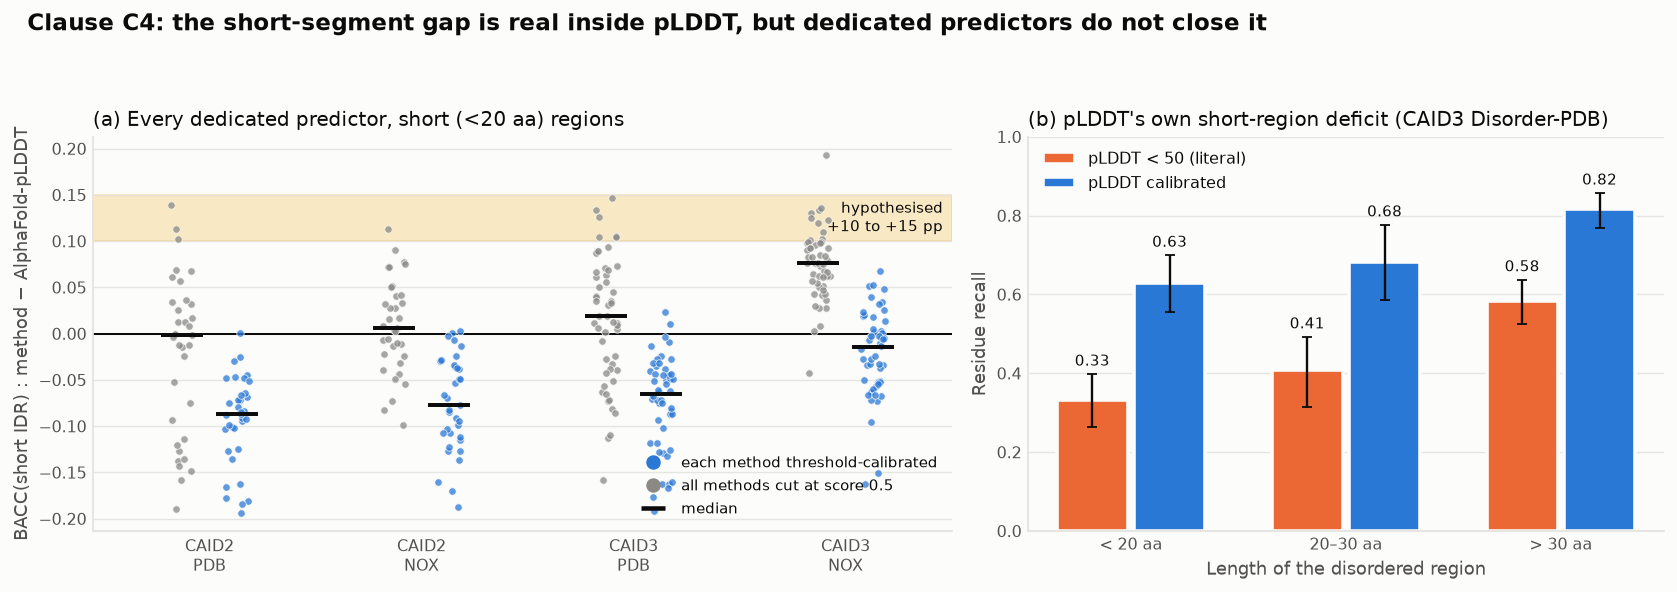
\includegraphics[width=0.95\linewidth]{figures/fig4_short_segment_claim.png}
    \caption{Per-method balanced-accuracy difference from \plddt on $<$20 aa disordered regions.
    The shaded band is the claimed $+10$ to $+15$\pp advantage. At calibrated thresholds the
    distribution sits below zero on every reference set and no method's CI clears zero; the same
    methods scored at a shared 0.5 cut populate the band. Both panels use identical residues and
    identical bootstrap resamples --- only the thresholds differ.}
    \label{fig:short}
\end{figure}

\subsection{Where \texorpdfstring{\plddt}{pLDDT} actually stands, fairly compared}
\label{sec:ranking}

Falsifying the folk claims cuts both ways. Calibrated and coverage-matched on the common target
set, \plddt is a respectable mid-pack disorder predictor (\tabref{tab:benchmark}): rank 9/37 and
11/56 on \dpdb, 16/37 and 17/56 on \dnox, comparable to IUPred3 and DISOPRED3, behind PUNCH2,
SETH-0 and the PredIDR family, ahead of flDPnn, ESpritz-D and MobiDB-lite. That is a
considerably more favourable verdict than the folk framing implies, and a considerably less
favourable one than ``\plddt $<$ 50 finds disorder'' implies. Calibration optimism is negligible:
the median gap between in-sample MCC-optimal \bacc and the $5\times2$-fold cross-validated
estimate is $0.20$--$0.66$\pp, with a maximum of $3.0$\pp across 186 method\,$\times$\,dataset
combinations, so the calibrated rankings are not an artefact of tuning on the evaluation data.

\begin{table}[t]
    \centering
    \small
    \resizebox{\textwidth}{!}{%
    \begin{tabular}{@{}lrlrlr@{}}
        \toprule
        \textbf{Reference set} & \textbf{\plddt \bacc} & \textbf{Rank} & \textbf{\plddt AUC} &
        \textbf{Best dedicated method} & \textbf{\afrsa \bacc} \\
        \midrule
        \caidtwo \dpdb   & 0.860 & 9 / 37  & 0.932 & PredIDR-long \textbf{0.887} & 0.886 \\
        \caidtwo \dnox   & 0.703 & 16 / 37 & 0.715 & SPOT-Disorder2 \textbf{0.734} & 0.713 \\
        \caidthree \dpdb & 0.871 & 11 / 56 & 0.943 & PUNCH2 \textbf{0.887} & 0.886 \\
        \caidthree \dnox & 0.789 & 17 / 56 & 0.833 & DisorderUnetLM \textbf{0.819} & 0.803 \\
        \bottomrule
    \end{tabular}}
    \caption{\plddt at its calibrated operating point against the full panel, coverage-matched.
    \plddt is mid-pack, not the outlier the folk rule's critics or its users assume; and \afrsa,
    derived from the same coordinates at no extra cost, is within a point of the best dedicated
    method on \dpdb.}
    \label{tab:benchmark}
\end{table}

\subsection{C3: \texorpdfstring{\plddt}{pLDDT} is a lossy readout of a structure that already knows better}
\label{sec:c3}

Four independent tests support the conflation mechanism.

\para{Test 1: same model, different readout.} \afrsa is the solvent accessibility of the
\emph{identical} AlphaFold2 coordinates, smoothed over a window. It beats \plddt on every
reference set: $\Delta$AUC $+0.015$ to $+0.056$ with $p \le 0.02$ throughout, and $\Delta$\bacc
$+0.017$ to $+0.044$ (\tabref{tab:readout}). This is the cleanest available test of the
conflation claim, because the structure model is held exactly fixed and only the quantity read
out of it changes. The confidence channel discards disorder-relevant information that is present
in the coordinates it is attached to.

\para{Test 2: a better folding model does not help.} AlphaFold3's \plddt is statistically
indistinguishable from AlphaFold2's on both \caidthree references ($p = 0.62$ and $0.61$), while
AlphaFold3's \emph{RSA} is significantly better ($+0.059$ AUC on \dnox, $p = 0.002$). If low
\plddt tracked genuine flexibility, a stronger folding model should sharpen it. It does not: the
gain lives in the readout, not in the model.

\begin{table}[t]
    \centering
    \small
    \resizebox{\textwidth}{!}{%
    \begin{tabular}{@{}llrrlrrr@{}}
        \toprule
        \textbf{Reference set} & \textbf{Comparison} & \textbf{$n$} & \textbf{$\Delta$AUC} &
        \textbf{95\% CI} & \textbf{$p$} & \textbf{$\Delta$\bacc} & \textbf{$p$} \\
        \midrule
        \caidtwo \dpdb   & AF2-RSA $-$ AF2-\plddt   & 299 & $\mathbf{+0.0160}$ & [$+0.0056$, $+0.0256$] & 0.002 & $+0.0263$ & 0.001 \\
        \caidtwo \dnox   & AF2-RSA $-$ AF2-\plddt   & 173 & $\mathbf{+0.0508}$ & [$+0.0201$, $+0.0894$] & 0.004 & $+0.0169$ & 0.032 \\
        \caidthree \dpdb & AF2-RSA $-$ AF2-\plddt   & 319 & $\mathbf{+0.0152}$ & [$+0.0032$, $+0.0311$] & 0.020 & $+0.0272$ & 0.001 \\
        \caidthree \dnox & AF2-RSA $-$ AF2-\plddt   & 204 & $\mathbf{+0.0561}$ & [$+0.0180$, $+0.0980$] & 0.002 & $+0.0435$ & 0.002 \\
        \midrule
        \caidthree \dpdb & AF3-\plddt $-$ AF2-\plddt & 319 & $-0.0021$ & [$-0.0102$, $+0.0082$] & 0.616 & $+0.0010$ & 0.856 \\
        \caidthree \dnox & AF3-\plddt $-$ AF2-\plddt & 204 & $+0.0072$ & [$-0.0150$, $+0.0341$] & 0.612 & $+0.0106$ & 0.356 \\
        \caidthree \dnox & AF3-RSA $-$ AF2-\plddt    & 204 & $\mathbf{+0.0585}$ & [$+0.0141$, $+0.1136$] & 0.002 & $+0.0513$ & 0.002 \\
        \bottomrule
    \end{tabular}}
    \caption{Controlled readout comparisons by paired bootstrap over targets. Changing the
    readout of a fixed AlphaFold2 model from confidence to geometry helps significantly
    everywhere; changing the folding model while keeping the confidence readout does not help at
    all.}
    \label{tab:readout}
\end{table}

\para{Test 3: residual signal inside \plddt strata.} Within the \plddt $<$ 50 stratum, \plddt
itself discriminates disorder at AUC $0.44$--$0.63$ --- at or below chance on the \dnox
references --- while RSA of the \emph{same} residues discriminates at $0.56$--$0.83$. In the
50--70 band the gap is widest (\plddt $0.56$--$0.68$ versus RSA $0.69$--$0.90$;
\tabref{tab:condinfo}, appendix). The confidence score saturates: once it has said ``not
confident'', it stops carrying information about how disordered a residue is, while the
structure still does (\figref{fig:mech}).

\para{Test 4: information overlap.} A 5-fold grouped-by-target cross-validated logistic probe on
the raw features --- an information probe, not a proposed predictor --- gives CV AUC 0.926/0.689/
0.931/0.761 for \plddt alone, 0.944/0.741/0.949/0.827 for RSA alone, and 0.949/0.743/0.956/0.822
for both. Adding \plddt on top of RSA gains at most $+0.007$ AUC and \emph{loses} $0.005$ on
\caidthree \dnox; adding RSA on top of \plddt gains $+0.023$ to $+0.065$. \plddt's disorder
information is very nearly a subset of the geometry's.

\begin{figure}[t]
    \centering
    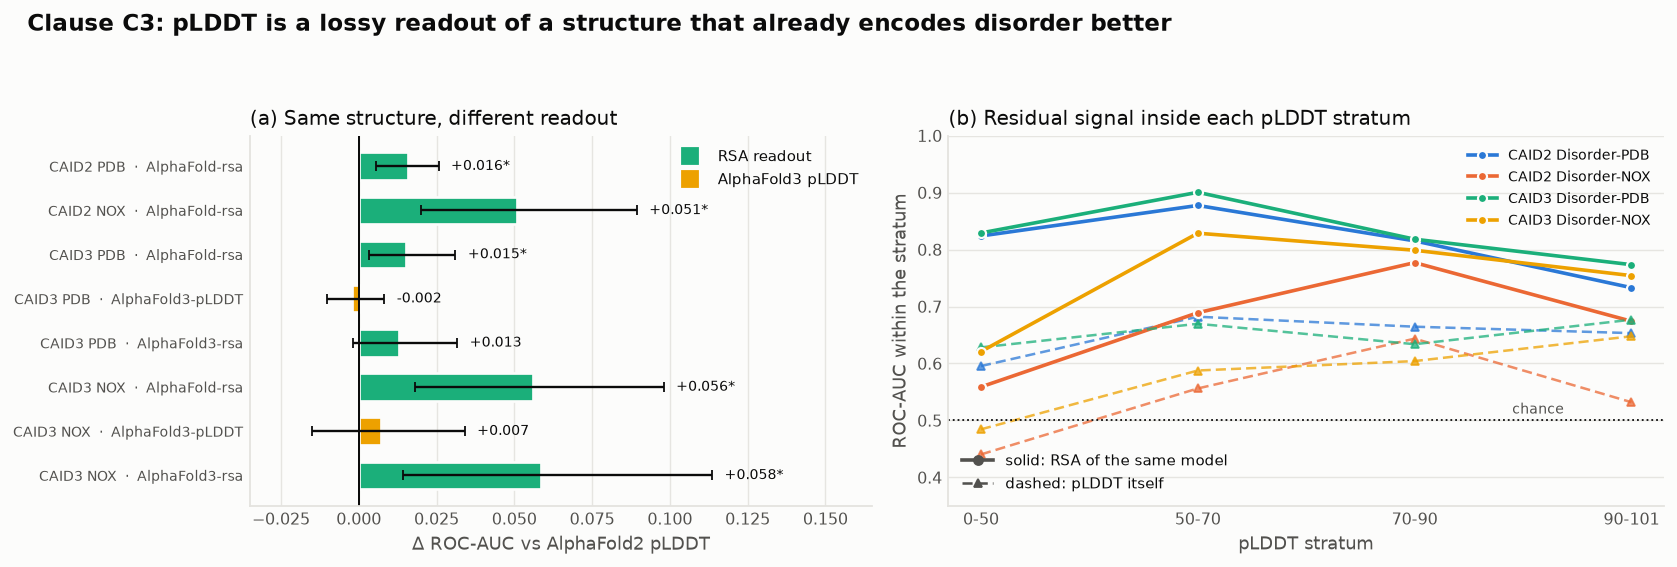
\includegraphics[width=0.95\linewidth]{figures/fig6_mechanism.png}
    \caption{The conflation mechanism. \captiona Reading solvent accessibility instead of
    confidence out of the same AlphaFold2 coordinates improves AUC on all four reference sets,
    while replacing AlphaFold2 with AlphaFold3 does not. \captionb Within \plddt strata, \plddt
    has saturated --- inside its own $<$50 band it discriminates disorder at chance level on the
    \dnox references --- while the geometry of the same model still separates disorder from
    order.}
    \label{fig:mech}
\end{figure}

\subsection{What the rule misses, structurally}
\label{sec:errors}

Decomposing the residues into true positives, false negatives, false positives and true
negatives (\tabref{tab:errorstrata}) shows what kind of disorder escapes the rule. The missed
disorder is \textbf{confidently modelled} --- mean \plddt 70--74, with 47--56\% of those residues
above \plddt 70 and 12--21\% above 90 --- and \textbf{solvent-exposed}, with mean RSA
$0.46$--$0.51$ against $0.25$--$0.31$ for true negatives, and only 17--23\% buried against
46--57\% of true negatives. It sits in shorter regions (median 110--161 aa versus 170--239 for
detected disorder) and has an intermediate amino-acid composition: detected disorder shows the
classic low-complexity signature (log$_2$ enrichment S $+0.64$, P $+0.58$, G $+0.55$, with strong
hydrophobic depletion I $-1.22$, W $-1.05$, F $-1.05$), whereas missed disorder keeps the
charged/proline enrichment (K $+0.44$, P $+0.35$, Q $+0.27$) but has no S/G enrichment
(S $-0.05$, G $-0.15$) and is only mildly hydrophobic-depleted (I $-0.37$).

\begin{table}[t]
    \centering
    \small
    \resizebox{\textwidth}{!}{%
    \begin{tabular}{@{}llrrrrr@{}}
        \toprule
        \textbf{Reference set} & \textbf{Stratum} & \textbf{$n$ residues} & \textbf{Mean \plddt} &
        \textbf{Mean RSA} & \textbf{\% buried} & \textbf{Median region len.} \\
        \midrule
        \multirow{4}{*}{\caidthree \dpdb}
          & TP (disordered, \plddt$<$50) & 18,037 & 37.0 & 0.638 & 2.7 & 170 \\
          & \textbf{FN (disordered, \plddt$\ge$50)} & 12,202 & \textbf{71.4} & \textbf{0.492} & \textbf{19.2} & \textbf{110} \\
          & FP (ordered, \plddt$<$50) & 886 & 41.4 & 0.547 & 13.9 & --- \\
          & TN (ordered, \plddt$\ge$50) & 62,840 & 91.9 & 0.255 & 56.1 & --- \\
        \midrule
        \multirow{2}{*}{\caidtwo \dpdb}
          & TP & 17,186 & 37.1 & 0.646 & 1.8 & 214 \\
          & FN & 10,428 & 73.5 & 0.463 & 23.2 & 125 \\
        \bottomrule
    \end{tabular}}
    \caption{Structural profile of the rule's error strata (2026 \afdb snapshot, Shrake--Rupley
    RSA). ``\% buried'' is the fraction with RSA $<$ 0.25. The disorder the rule misses is not
    borderline: it is confidently modelled and mostly solvent-exposed, \ie extended
    pseudostructure rather than genuinely ambiguous prediction.}
    \label{tab:errorstrata}
\end{table}

This decomposes the failure into two mechanisms with different remedies. The 17--23\% buried
fraction is \textbf{conditional folding}~\citep{alderson2023}: AlphaFold confidently builds a
folded conformation for a region that is disordered in isolation, and no confidence threshold
can recover it. The larger, exposed fraction is \textbf{pseudostructure}~\citep{richardson2025}:
AlphaFold confidently models an extended or helical conformation for a region that is genuinely
flexible. That fraction \emph{is} recoverable --- it is exactly what the RSA readout catches, and
it is why RSA beats \plddt (\figref{fig:errors}).

\begin{figure}[t]
    \centering
    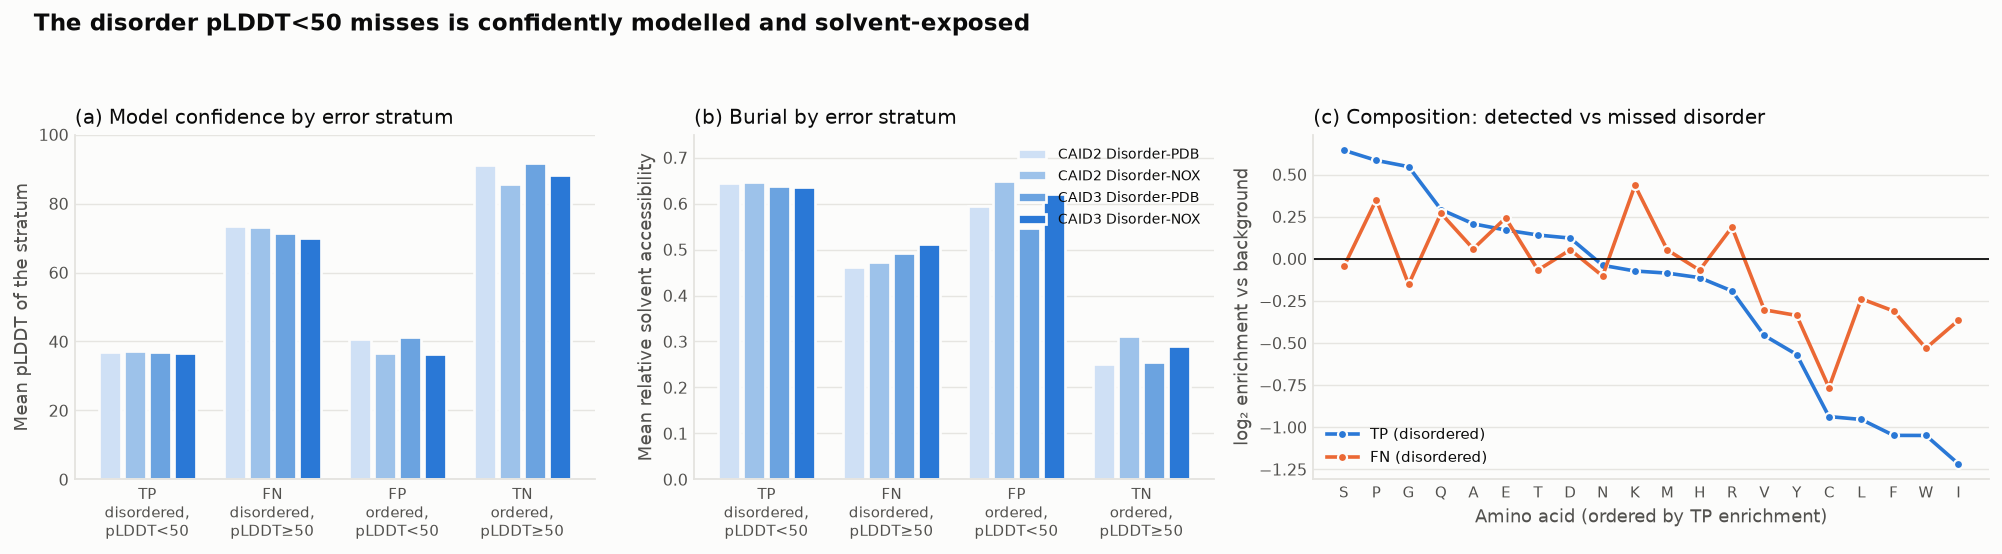
\includegraphics[width=0.95\linewidth]{figures/fig7_error_strata.png}
    \caption{What \plddtrule misses. \captiona Confidence distribution by stratum: false
    negatives are not clustered just above the cutoff but spread across the confident range.
    \captionb Solvent accessibility separates false negatives from true negatives even where
    confidence does not. \captionc Amino-acid composition places missed disorder between
    canonical low-complexity \idrs and ordered sequence, consistent with a conformation
    AlphaFold can commit to.}
    \label{fig:errors}
\end{figure}

\section{Discussion}
\label{sec:discussion}

\subsection{Interpretation}

The audited claim is best read as three empirical predictions plus one causal story, and the
data separate them cleanly.

\para{The two point predictions are wrong for instructively different reasons.} \cone is wrong
because the rule is \emph{conservative}, not liberal: it sits roughly 20 \plddt units below the
disorder-optimal operating point and captures only the 19--40\% of residues in the lowest
confidence band. The framing appears to assume that ``very low confidence'' is a permissive
filter; it is a strict one. \ctwo is wrong in a deeper way, because it is not a statement about
AlphaFold at all. The same predictions, the same residues and the same threshold give
specificity 0.98 or 0.67 depending on whether the benchmark counts X-ray-missing residues as
negatives. A claim whose truth value flips on an annotation convention is under-specified, and
the fix is simply to state the convention.

\para{The comparative prediction is wrong in the opposite direction, and its origin is
diagnosable.} Once thresholds are calibrated, \plddt is \emph{better} than the median dedicated
predictor on short segments, on all four datasets, under both a strict and a generous
definition, with zero significant exceptions among 174 comparisons. The claim is nonetheless
recoverable at a shared 0.5 threshold, where it is not only true but quantitatively accurate.
We think this is how the belief arises, and the lesson generalises: whenever a comparison mixes
a method whose scores are physically anchored (\plddt is a predicted lDDT, so 0.5 means
something specific about geometry) with methods whose scores are arbitrary monotone confidences,
a shared cut compares operating points rather than methods.

\para{The causal story is right, and more specific than usually stated.} Four independent tests
support conflation: RSA of the same coordinates beats \plddt on every reference set; a stronger
folding model does not improve \plddt but does improve RSA; inside the low-\plddt stratum \plddt
is at chance while RSA is not; and \plddt adds at most $+0.007$ AUC on top of RSA while RSA adds
up to $+0.065$ on top of \plddt. The error-stratum analysis sharpens ``conflation'' into a
concrete failure mode: \plddt is high wherever AlphaFold commits to \emph{a} conformation,
whether or not that conformation is real. Most missed disorder is confidently modelled and
solvent-exposed --- extended pseudostructure --- which is why a geometric readout rescues it and
why raising the confidence threshold only partially helps.

\subsection{Comparison with prior work}

Our AUCs reproduce the official CAID values to three decimals wherever coverage is complete
(\secref{sec:validation}), so the study is anchored to the published assessment. Relative to
\citet{kurgan2023}, who report AF2-\plddt at AUC 0.722 and AF2-RSA at 0.768 on CAID1, we find
higher absolute AUCs on \caidtwo/\caidthree \dpdb (0.929--0.934 and 0.944--0.950) but the same
ordering and a similar gap. The absolute difference is a reference-set effect: CAID1 differs
from CAID2/3, and \dpdb's exclusion of X-ray-missing negatives raises all AUCs. Their
protein-level finding that short-\idr proteins are harder is reproduced here at region level and
shown to be a property of \emph{all} methods rather than a \plddt-specific weakness. We also
confirm the CAID3 observation that \afthreeplddt does not improve on \afplddt, and add that the
difference is not statistically distinguishable from zero.

\subsection{Practical recommendations}

\begin{itemize}[leftmargin=*,itemsep=1pt,topsep=2pt]
    \item \textbf{Do not use \plddtrule as a disorder detector if recall matters.} Use
    \plddt $<$ 70 (the MCC-optimal region is 69--72), which raises recall on long regions from
    $\approx$0.60 to 0.78--0.85 at specificity $\ge$ 0.95 on \dpdb.
    \item \textbf{Prefer \afrsa to \afplddt.} It costs nothing extra, since the structure is
    already computed, and it is significantly better on every reference set tested.
    \item \textbf{State the negative-set convention} whenever reporting specificity or precision
    for a disorder predictor. Reporting one convention silently determines the answer.
    \item \textbf{Never compare disorder predictors at a shared score threshold.} This paper
    contains a worked example of the false conclusion that follows.
\end{itemize}

\subsection{Limitations}

\para{Methodological.} Our primary ``calibrated'' operating point maximises MCC on the full
data, following CAID's own convention, and is therefore optimistically biased. We measured the
optimism by $5\times2$-fold cross-validation over targets and found it small (median
$0.20$--$0.66$\pp, max $3.0$\pp), but it is not zero and is slightly larger on the \dnox
references where the class balance is less favourable. Balanced accuracy on a length stratum is
a constructed quantity that the folk claim does not define; we report two definitions that
bracket the reasonable range and agree, but a third could disagree. Our $p$-values are
percentile-bootstrap rather than exact, which can be slightly anti-conservative for small
effects; the \cfour conclusion rests on effects of the wrong \emph{sign}, so this is not
load-bearing there, but it matters for the marginal AlphaFold3 comparisons, which we report as
null rather than as equivalence. We apply no multiple-comparison correction across the 174 \cfour
comparisons; correction would only strengthen the ``0 better'' conclusion and weaken the ``97
worse'' one, so we report both counts and lean on the former.

\para{Data and scope.} CAID1 is no longer retrievable, so \citet{kurgan2023} cannot be
reproduced exactly on their own data; CAID2 and CAID3 v3 supersede it. The ground truth is
\disprot-derived and inherits \disprot's biases: curation is literature-driven and long,
well-characterised \idrs are over-represented relative to short ones (1,610--1,808 residues in
$<$20 aa regions versus 16,502--19,703 in $>$30 aa regions), so short-region estimates are
correspondingly noisier, as the wider CIs in \tabref{tab:strata} show. Coverage matching costs
18--36\% of targets because the intersection is set by the worst-covered panel member; the
clause tests are therefore also reported on \plddt's own coverage and on the full reference,
with unchanged conclusions. Absence of annotation is not annotation of order --- \dnox assumes it
is, \dpdb refuses to --- and neither is a gold standard, which is exactly why both are reported.
Our re-parsed \afdb coordinates differ from the CAID-era models at $r = 0.992$ (median 1.14
\plddt units), which affects only the descriptive error-stratum statistics, not the benchmark
results; likewise the structural analysis uses Shrake--Rupley rather than DSSP accessibility,
while the benchmark comparisons use the official DSSP-based \afrsa submissions. Finally, the
2-feature logistic probe is linear, so ``\plddt adds $\le 0.007$ on top of RSA'' is a statement
about linearly accessible information, not an information-theoretic bound. We did not test
predicted aligned error, MSA depth, or per-domain analyses.

\para{What could invalidate these results.} A ground truth in which short disordered regions are
systematically better represented could change the \cfour magnitudes, though we doubt it would
change the sign given the size and consistency of the effect. A demonstration that CAID's
\afplddt submission used a non-standard AlphaFold configuration would undercut the mapping to
the folk rule; we checked this as far as the data allow ($r = 0.992$ against \afdb) and found no
evidence of it. And if a reader's operational definition of ``disordered'' is ``not resolved in
a crystal'', then \dnox is the wrong reference for them and the specificity story changes ---
which is itself the paper's central methodological point.

\subsection{Broader implications}

Two lessons travel beyond disorder prediction. First, a benchmark that publishes more than one
convention for what counts as a negative is publishing more than one question, and a claim
stated without naming the convention has no truth value. Second, a folk rule inherited from a
model's internal diagnostic is unlikely to be calibrated for a downstream task it was never
trained on: \plddt targets lDDT-C$\alpha$, not disorder, and the 50 boundary comes from
AlphaFold's own confidence banding, not from any disorder annotation. Both failure modes are
easy to reproduce in other settings where a model's uncertainty output gets repurposed as a
semantic label.

\section{Conclusion}
\label{sec:conclusion}

We audited the rule ``AlphaFold2 \plddt $<$ 50 means intrinsically disordered'' at the operating
point at which it is actually used, on the CAID round-2 and round-3 blind assessments, under
both official reference conventions, against 35--52 dedicated disorder predictors.

\para{Findings.} \plddtrule does not identify disordered regions with sensitivity above 0.8: it
achieves $0.60$--$0.63$ overall and $0.63$--$0.65$ on regions longer than 30 aa, missing roughly
40\% of experimentally annotated disorder, with $P(\text{sens} \ge 0.80) = 0.000$ in every
setting tested. Its specificity is 0.98 or 0.67--0.76 depending purely on whether the benchmark
counts X-ray-missing residues as negatives, so the ``specificity $<$ 0.7'' clause describes an
annotation convention rather than a predictor. Dedicated predictors do not achieve 10--15\%
better balanced accuracy on short segments: after fair threshold calibration, none of them is
significantly better and the median is $1.5$--$8.7$ points \emph{worse}; the claimed gap is
reproducible only when all methods are cut at a shared, arbitrary threshold. The mechanism,
however, is correct and can be demonstrated directly: \plddt conflates flexibility with model
confidence, which is why reading solvent accessibility out of the same AlphaFold2 coordinates is
significantly better on every reference set, and why the disorder \plddt misses is confidently
modelled and solvent-exposed.

\para{Takeaway.} \plddtrule is a high-precision, low-recall disorder detector, and only under
the \dpdb negative-set convention. Raise the cutoff to $\approx$70 if recall matters, prefer the
free geometric readout of the same model, and state which negative-set convention you mean.

\para{Future work.} Three directions follow directly. The 77--83\% of missed disorder that is
not buried should be recoverable by a rule combining \plddt with local RSA and secondary-structure
content; quantifying the ceiling of that combination would say how much of the gap is closable
without leaving the AlphaFold model. The buried false negatives should be cross-referenced
against curated conditionally folded \idr sets~\citep{alderson2023} to check that they are the
same population, and tested against partner-aware predictions. And predicted aligned error is
the natural next signal, since a residue can carry high \plddt locally while being poorly
positioned relative to the rest of the chain --- which is exactly the pseudostructure signature.
Two questions remain open: whether the \plddt saturation we observe below 50 is intrinsic to the
lDDT target or an artefact of how AlphaFold's confidence head is trained, and whether a benchmark
can be built whose negatives are defined by positive experimental evidence of order rather than
by absence of evidence of disorder. Both CAID conventions are proxies for a reference set that
nobody has built.


\bibliography{references}

\appendix
\section{Robustness to the target-set convention}
\label{sec:app_robustness}

Clauses \cone and \ctwo concern \plddt alone and should not be hostage to other panel members'
coverage. \tabref{tab:robustness} repeats the clause tests under three target-set conventions:
the intersection of targets covered by every panel method (used for all method comparisons),
\plddt's own coverage (used in \tabref{tab:clause}), and the full reference with targets absent
from \afdb scored as all-ordered. \caidthree has full AlphaFold coverage, so its last two rows
coincide. Sensitivity spans $0.51$--$0.63$; the pessimistic convention lowers it, and nothing
raises it near 0.8.

\begin{table}[h]
    \centering
    \small
    \resizebox{\textwidth}{!}{%
    \begin{tabular}{@{}llrrrrrrr@{}}
        \toprule
        \textbf{Reference set} & \textbf{Target set} & \textbf{$n$} & \textbf{Sens.} &
        \textbf{Sens $>$30} & \textbf{Sens $<$20} & \textbf{Spec.} & \textbf{\bacc} & \textbf{AUC} \\
        \midrule
        \multirow{3}{*}{\caidtwo \dpdb}
          & panel intersection & 240 & 0.576 & 0.598 & 0.393 & 0.988 & 0.782 & 0.932 \\
          & \plddt own coverage & 299 & 0.610 & 0.634 & 0.416 & 0.986 & 0.798 & 0.929 \\
          & all targets, missing $=$ ordered & 348 & 0.511 & 0.528 & 0.366 & 0.989 & 0.750 & 0.810 \\
        \midrule
        \multirow{3}{*}{\caidtwo \dnox}
          & panel intersection & 135 & 0.575 & 0.583 & 0.433 & 0.712 & 0.644 & 0.715 \\
          & \plddt own coverage & 173 & 0.620 & 0.630 & 0.429 & 0.673 & 0.646 & 0.695 \\
          & all targets, missing $=$ ordered & 210 & 0.511 & 0.520 & 0.332 & 0.788 & 0.649 & 0.692 \\
        \midrule
        \multirow{2}{*}{\caidthree \dpdb}
          & panel intersection & 261 & 0.551 & 0.583 & 0.331 & 0.987 & 0.769 & 0.943 \\
          & \plddt own coverage / all targets & 319 & 0.599 & 0.630 & 0.349 & 0.980 & 0.790 & 0.934 \\
        \midrule
        \multirow{2}{*}{\caidthree \dnox}
          & panel intersection & 161 & 0.588 & 0.608 & 0.250 & 0.835 & 0.712 & 0.833 \\
          & \plddt own coverage / all targets & 204 & 0.629 & 0.648 & 0.264 & 0.761 & 0.695 & 0.778 \\
        \bottomrule
    \end{tabular}}
    \caption{Clause tests under three target-set conventions. The conclusion for \cone is
    unchanged in all cases.}
    \label{tab:robustness}
\end{table}

\section{Region-level detection rates}
\label{sec:app_regions}

The folk rule is phrased about regions, so \tabref{tab:regiondetect} reports region-level
detection: a region counts as detected when at least a given fraction of its evaluated residues
is predicted disordered at the literal cut. The length ordering of \secref{sec:c4} survives at
every overlap criterion.

\begin{table}[h]
    \centering
    \small
    \resizebox{\textwidth}{!}{%
    \begin{tabular}{@{}lrrrrrrr@{}}
        \toprule
        \textbf{Reference set} & \textbf{Min overlap} & \textbf{Det.\ $<$20 aa} & \textbf{$n$} &
        \textbf{Det.\ 20--30 aa} & \textbf{$n$} & \textbf{Det.\ $>$30 aa} & \textbf{$n$} \\
        \midrule
        \multirow{3}{*}{\caidtwo \dpdb}
          & 0.25 & 0.737 & 118 & 0.797 & 64 & \textbf{0.869} & 153 \\
          & 0.50 & 0.661 & 118 & 0.719 & 64 & \textbf{0.797} & 153 \\
          & 0.75 & 0.576 & 118 & 0.625 & 64 & \textbf{0.641} & 153 \\
        \midrule
        \multirow{3}{*}{\caidtwo \dnox}
          & 0.25 & 0.871 & 31 & 0.808 & 26 & \textbf{0.932} & 117 \\
          & 0.50 & 0.806 & 31 & 0.769 & 26 & \textbf{0.863} & 117 \\
          & 0.75 & \textbf{0.774} & 31 & 0.654 & 26 & 0.701 & 117 \\
        \midrule
        \multirow{3}{*}{\caidthree \dpdb}
          & 0.25 & 0.772 & 136 & 0.797 & 64 & \textbf{0.907} & 172 \\
          & 0.50 & 0.647 & 136 & 0.750 & 64 & \textbf{0.831} & 172 \\
          & 0.75 & 0.544 & 136 & 0.547 & 64 & \textbf{0.686} & 172 \\
        \midrule
        \multirow{3}{*}{\caidthree \dnox}
          & 0.25 & 0.750 & 44 & 0.844 & 32 & \textbf{0.939} & 131 \\
          & 0.50 & 0.591 & 44 & 0.781 & 32 & \textbf{0.893} & 131 \\
          & 0.75 & 0.523 & 44 & 0.625 & 32 & \textbf{0.740} & 131 \\
        \bottomrule
    \end{tabular}}
    \caption{Region-level detection rate of \plddtrule by region length and overlap criterion.}
    \label{tab:regiondetect}
\end{table}

\section{Conditional information within \texorpdfstring{\plddt}{pLDDT} strata}
\label{sec:app_condinfo}

\tabref{tab:condinfo} reports, within each \plddt band, how well the solvent accessibility of the
same model separates disordered from ordered residues, together with the cross-validated logistic
probes of \secref{sec:c3}. Inside the $<$50 band --- where the confidence signal has saturated and
discriminates at AUC $0.44$--$0.63$ --- the geometry of the same model still reaches
$0.56$--$0.83$.

\begin{table}[h]
    \centering
    \small
    \begin{tabular}{@{}lrrrrrrr@{}}
        \toprule
        & \multicolumn{4}{c}{\textbf{AUC(RSA) within \plddt band}} & \multicolumn{3}{c}{\textbf{5-fold CV logistic probe}} \\
        \cmidrule(lr){2-5} \cmidrule(lr){6-8}
        \textbf{Reference set} & \textbf{0--50} & \textbf{50--70} & \textbf{70--90} & \textbf{90--100} &
        \textbf{\plddt} & \textbf{RSA} & \textbf{both} \\
        \midrule
        \caidtwo \dpdb   & 0.824 & 0.877 & 0.815 & 0.733 & 0.9263 & 0.9440 & \textbf{0.9490} \\
        \caidtwo \dnox   & 0.559 & 0.689 & 0.777 & 0.674 & 0.6888 & 0.7405 & \textbf{0.7431} \\
        \caidthree \dpdb & 0.829 & 0.901 & 0.818 & 0.773 & 0.9314 & 0.9488 & \textbf{0.9555} \\
        \caidthree \dnox & 0.621 & 0.829 & 0.799 & 0.754 & 0.7613 & \textbf{0.8267} & 0.8218 \\
        \bottomrule
    \end{tabular}
    \caption{Residual disorder signal in AlphaFold2 geometry, conditioned on confidence. Adding
    \plddt on top of RSA gains at most $+0.007$ AUC and loses $0.005$ on \caidthree \dnox, while
    adding RSA on top of \plddt gains $+0.023$ to $+0.065$.}
    \label{tab:condinfo}
\end{table}

\section{Calibration optimism}
\label{sec:app_optimism}

Our primary operating point selects each method's MCC-optimal threshold on the evaluation data.
\tabref{tab:optimism} quantifies the resulting optimism by repeated $5\times2$-fold
cross-validation over targets: the median gap is $0.20$--$0.66$ percentage points of balanced
accuracy, with a maximum of $3.0$\pp over 186 method\,$\times$\,dataset combinations. The
calibrated rankings in \secref{sec:ranking} are therefore not an artefact of tuning on the
evaluation data.

\begin{table}[h]
    \centering
    \small
    \resizebox{\textwidth}{!}{%
    \begin{tabular}{@{}lrrrrr@{}}
        \toprule
        \textbf{Reference set} & \textbf{$n$ methods} & \textbf{Median in-sample \bacc} &
        \textbf{Median CV \bacc} & \textbf{Median optimism (pp)} & \textbf{Max optimism (pp)} \\
        \midrule
        \caidtwo \dpdb   & 37 & 0.8175 & 0.8125 & 0.281 & 1.367 \\
        \caidtwo \dnox   & 37 & 0.7000 & 0.6848 & 0.663 & 3.036 \\
        \caidthree \dpdb & 56 & 0.8272 & 0.8255 & 0.196 & 1.691 \\
        \caidthree \dnox & 56 & 0.7625 & 0.7571 & 0.339 & 2.524 \\
        \bottomrule
    \end{tabular}}
    \caption{In-sample versus cross-validated calibrated balanced accuracy.}
    \label{tab:optimism}
\end{table}

\section{Full panel ranking}
\label{sec:app_ranking}

\Figref{fig:ranking} shows the calibrated, coverage-matched ranking of the whole panel on all
four reference sets, with \plddt and the AlphaFold-derived controls highlighted. \Figref{fig:calib}
shows the empirical probability of disorder as a function of \plddt bin, which is the graphical
form of \tabref{tab:calibration}.

\begin{figure}[h]
    \centering
    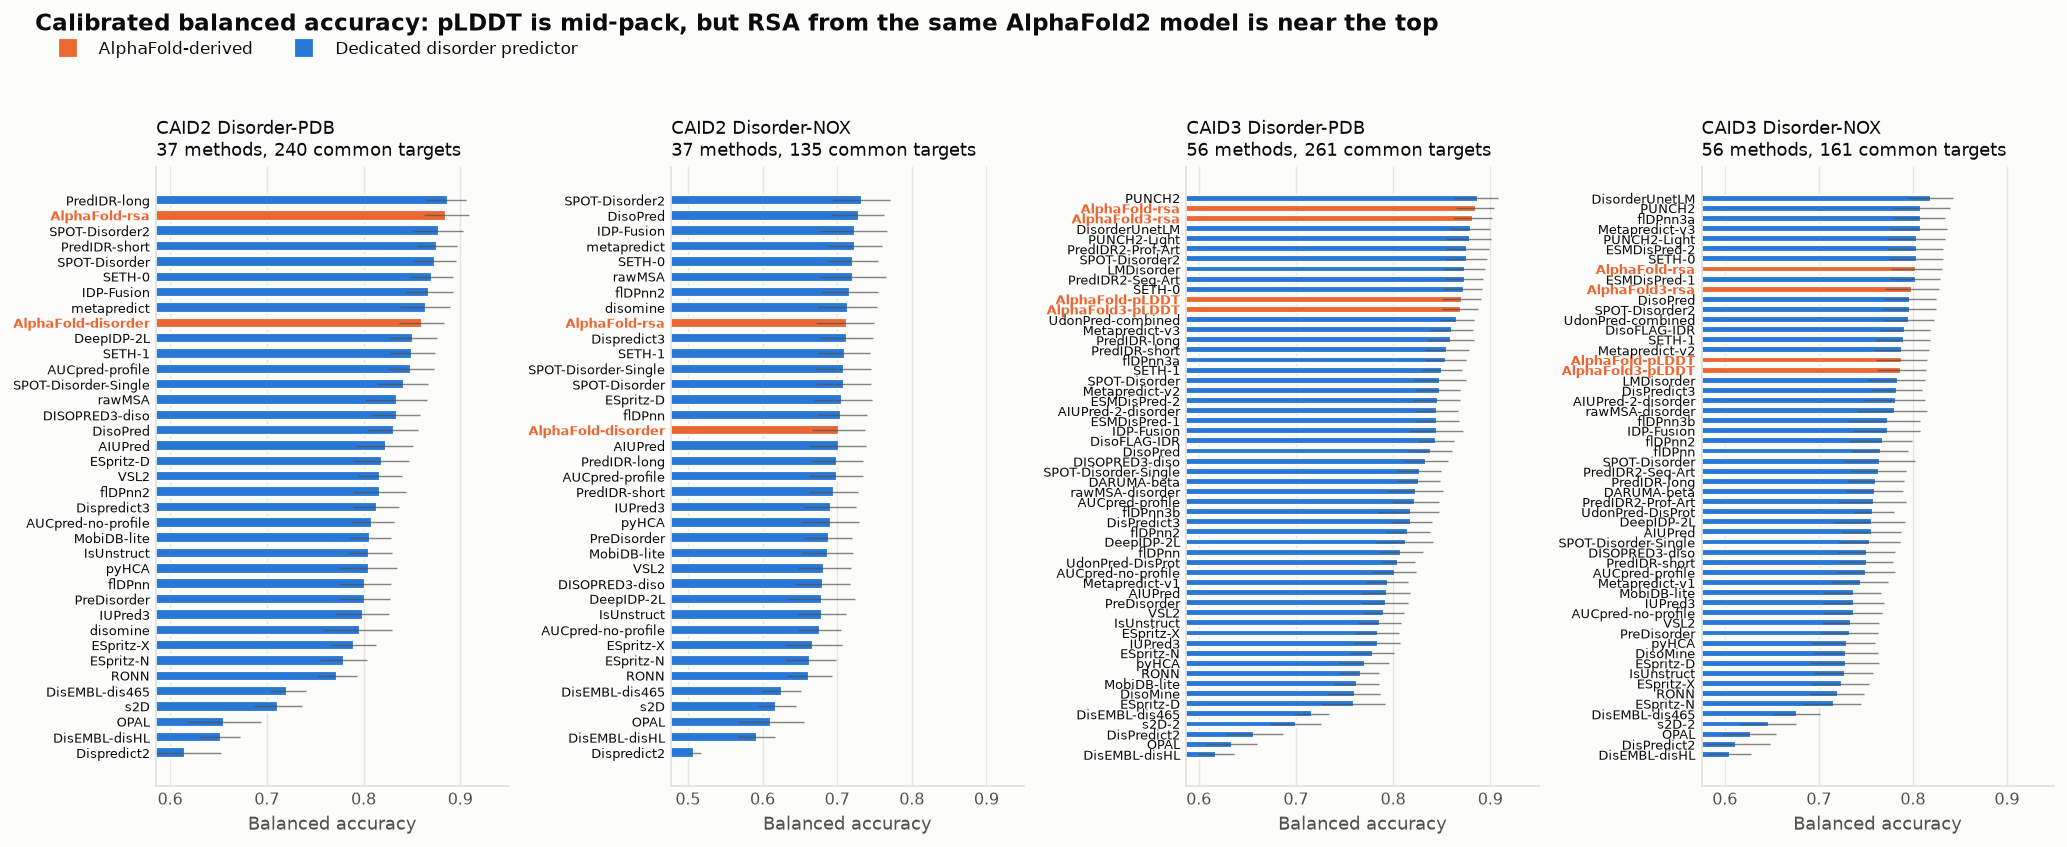
\includegraphics[width=0.92\linewidth]{figures/fig3_benchmark_ranking.png}
    \caption{Calibrated balanced accuracy of every panel method on the coverage-matched target
    sets. \plddt is mid-pack on all four references; \afrsa, read from the same coordinates, is
    consistently near the top.}
    \label{fig:ranking}
\end{figure}

\begin{figure}[h]
    \centering
    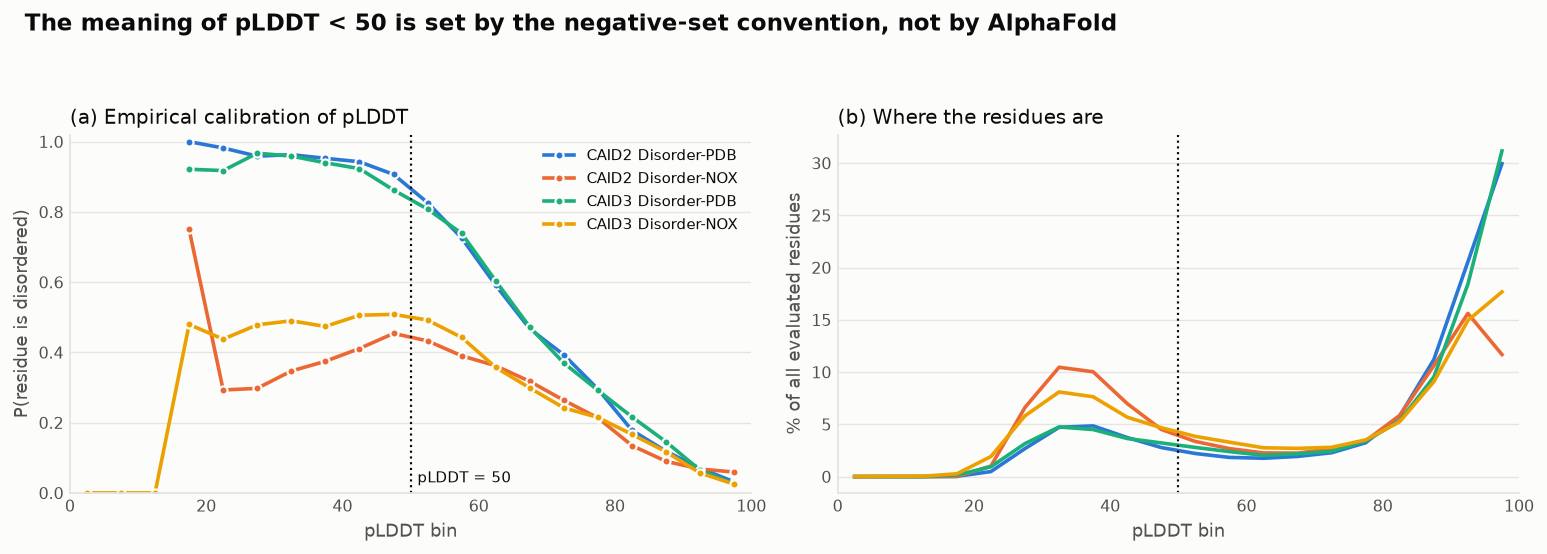
\includegraphics[width=0.92\linewidth]{figures/fig5_calibration.png}
    \caption{Empirical probability that a residue is annotated disordered, as a function of its
    \plddt bin. The curves for the two negative-set conventions are shifted by roughly a factor
    of two in precision at every bin, while the fraction of all disorder falling below \plddt 50
    is nearly identical.}
    \label{fig:calib}
\end{figure}


\end{document}
